\section{Periodic Event Handling Module}
\label{sec:periodic}
Periodic event Handling Module(periodic module in short) manages periodic events such as route refresh requests and periodic status messages.
This module has two threads:
\begin{itemize}
%\item{Periodically writes sessions status trigger message (type 3) into label queue if configured.}
\item{\emph{Periodic Status Messages Thread:} It periodically writes session status messages(BMF type 5), queues status messages(BMF type 6) and chains status messages(BMF type 7) into label queue if configured.}
\item{\emph{Route Refresh Request Thread:} It centralized schedules and executes the route refreshes for all the peers if configured. For each peer, there are two possibilities. }
	\begin{itemize}
		\item{If this peer supports route refresh, periodic module will notify peering module to send route refresh request to the peer.}
		\item{If this peer doesn't support route refresh, periodic module will simulate route refresh by sending local stored RIB-IN out.}
	\end{itemize}
\end{itemize}

The main data structure of periodic event handling module has five fields:
\begin{itemize}
%\item{\emph{sessionsStatusTriggerInt:} It indicates the interval of sending sessions status trigger messages. It is set by configuration module and read by periodic module. }
\item{\emph{StatusMessageInterval:} It indicates the interval of sending periodic status messages for peering sessions, queues and chains. It is configured by user. }
%\item{\emph{sessionsStatusTriggerTimer:} It indicates when is the next time to send sessions status trigger message. It is set and read by periodic module. }
\item{\emph{RouteRefreshInterval:} It indicates the interval of requesting route refresh for every peer that is configured for route refresh. It is configured by user }

%\item{\emph{sessions:} It is a pointer to an array of session structures for all the peers. It is set by configuration module and read by periodic module.}
%\item{\emph{RLs:} It is a pointer to an array of rib and labeling structures for all the peers. It is set by configuration module and read by periodic module.}
\item{\emph{labelQueueWriter:} It is used to write messages into the label queue.}
\item{\emph{shutDownFlag:} It is used to signal periodic module to exit. Specifically both threads keep checking this flag, they will quit if it becomes TRUE.}
\end{itemize}
%\item{\emph{routeRefreshes:} It is a array of RouteRefresh structures. Each session(peer) is attached with one RouteRefresh structure. Each RouteRefresh consists of three field.}
%	\begin{itemize} 
%		\item{\emph{sessionID:} It is a 16 bit session identification. It is set by configuration module and read by periodic module.}
%		\item{\emph{routeRefreshInt:} It indicates the interval of route refresh for this session(peer). It is set by configuration module and read by periodic module.}
%		\item{\emph{routeRefreshTimer:} It indicates the next scheduled route refresh time. It is only used by periodic module. }
%	\end{itemize}
%\end{itemize}
%For the details of this structure, see Figure\ref{fig:PeriodicModuleStruct}.
%\begin{figure*}
%\centering
%\scalebox{1}{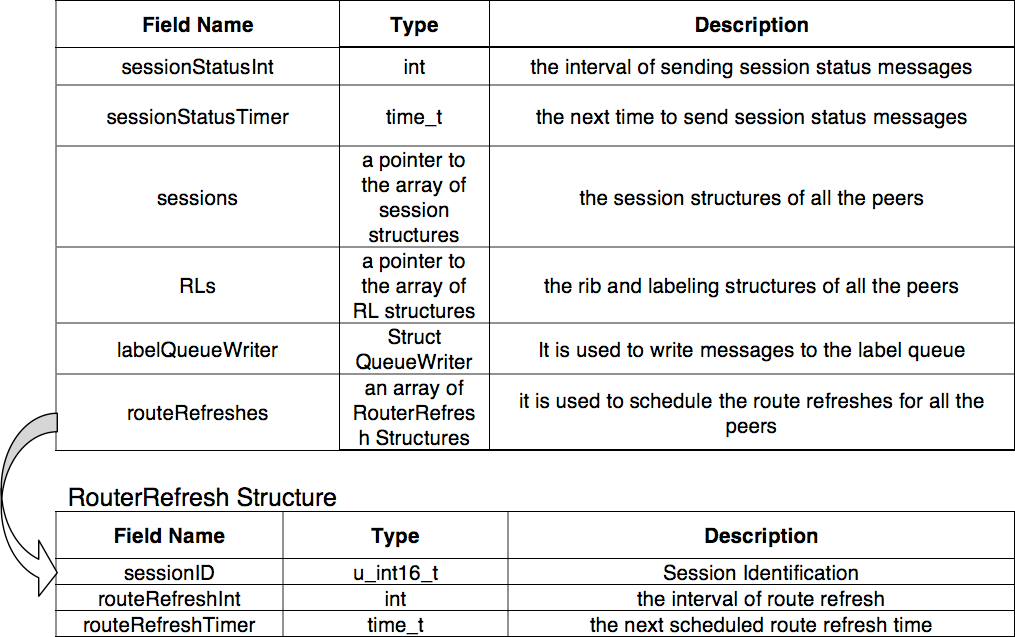
\includegraphics{figs/PeriodicModuleStruct.pdf}}
%\caption{Data Structure of Periodic Event Handling Module}
%\label{fig:PeriodicModuleStruct}
%\end{figure*}
Next we will discuss the detail of the two threads.

\subsection{Periodic Status Messages Thread}
%\subsubsection{ Session Status Message Format}
This thread writes one status message for each peering session, one status message fro all queues and one status message for all chains into the label queue every 'StatusMessageInterval' interval.  Peering session status message (BMF type 5) only includes a session ID instead of including the detail information. Queues' status message(BMF type 6) and chains' status message(BMF type 7) are not associated with a particular peering session.

Then when XML module reads a session status message from label queue, it will extract the session ID from it and retrieve the detail information based on the session ID. Finally the detail information of a peering session will be converted to XML and write into a XML queue. The detail is built from peering session structure( see section \ref{sec:peering:sessionstructure}).  More specifically, it consists of the follow fields:
%\begin{itemize}
%\item{\emph{fsm\_state:} is the current state of FSM that could be one of the six values: Idle, Connect, Active, OpenSent, OpenConfirm and Etablished.  }
%\item{\emph{last\_action:} is a timestamp that indicates when the last action of a peering session is.}
%\item{\emph{establish\_time:} is a timestamp that indicates when the peering session gets established. }
%\item{\emph{message\_rcvd:} is the number of received BGP messages. }
%\item{\emph{prefix\_count:} is the number of prefixes in RIB-IN table. }
%\item{\emph{attribute\_count:} is the number of unique attributes sets in RIB-IN table. }
%\item{\emph{connect\_retry\_count:} is the number of times to retry a tcp connection. }
%\item{\emph{session\_down\_count:} is the number of times BGP session goes down. }
%\item{\emph{session\_last\_down:} is a timestamp that indicated when BGP session went down last time. }
%\end{itemize}
When XML module reads a queues status message from label queue, it will ignore the session ID from it and retrieve the status information all queues. Finally the status information of all peers will be converted to XML and write into a XML queue. Similarly when XML module reads a chains status message from label queue, it will ignore the session ID from it and retrieve the status information all chains.
For the XML format of these periodic status messages, please refer to the XML specification.

%\begin{itemize}
%\item{\emph{FSM Info:} It contains 'state', 'keepaliveInt', 'holdTime', 'routeRefreshType' from FSM substructure in session structure and 'routerRefreshInt' from RouteRefresh Structure. }
%\item{\emph{Session Stats:} It contains all the fields from statistics substructure in session structure.}
%\item{\emph{RIB and Label Stats:} It contains all the stats related fields from RL structure.}
%\end{itemize}
%For the details of session status message, see Figure\ref{fig:SessionStatusStruct}.
%\begin{figure*}
%\centering
%\scalebox{1}{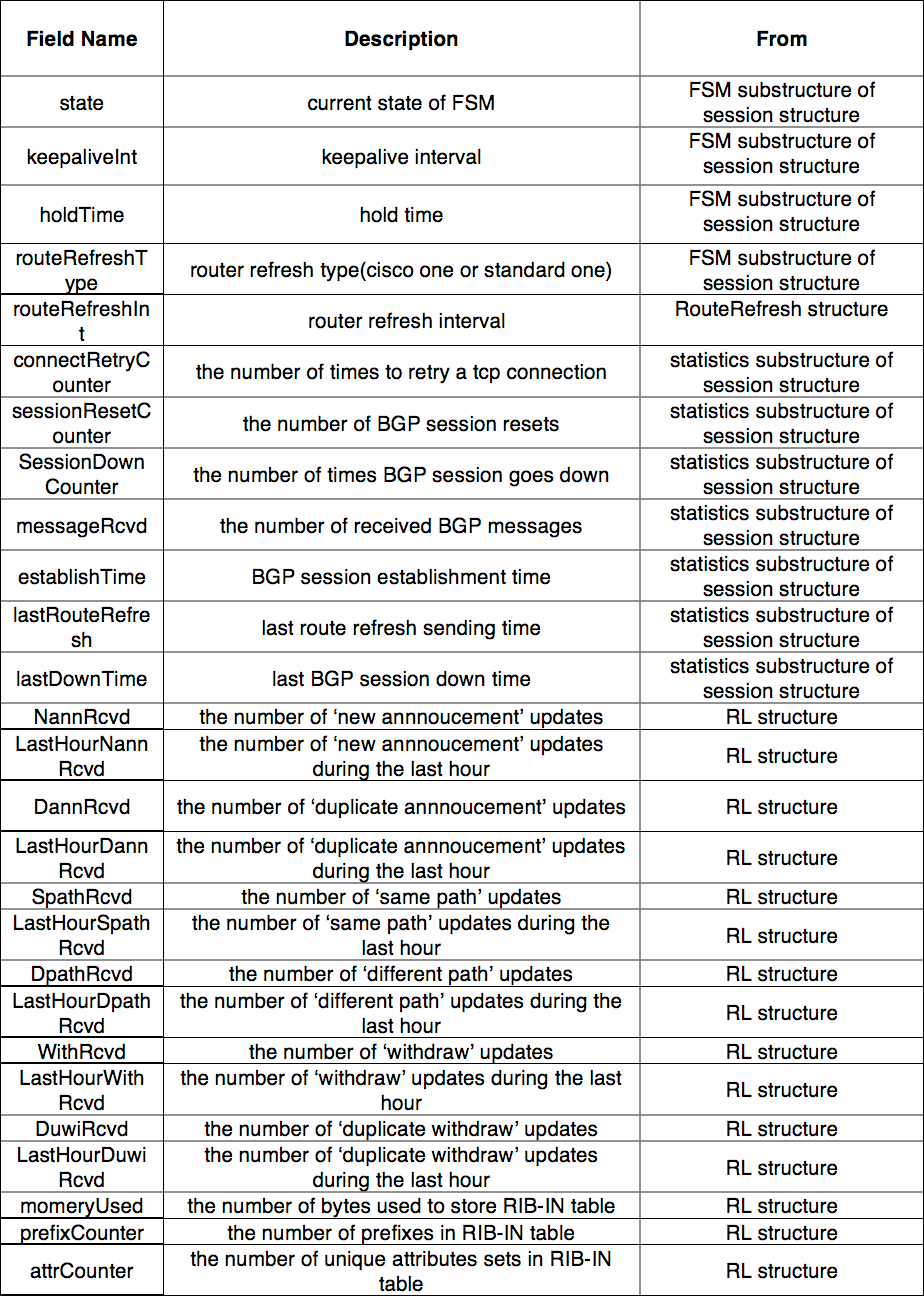
\includegraphics{figs/SessionStatusStruct.pdf}}
%\caption{Data Field of Session Status Message}
%\label{fig:SessionStatusStruct}
%\end{figure*}

%\subsubsection{Send Session Status Messages}

%The 'sessionStatusTimer' field works as a timer to send session status messages for all the peers. When it is timed out, the periodic module will first retrieve all the sessions based on the 'sessions' field in its data structure. Then for each session, the periodic module does the following:
%\begin{itemize}
%\item{Based on its session ID, locate the corresponding RL structure from 'RLs' field in its main data strcutrure.}
%\item{Based on its session ID, locate the corresponding RouteRefresh structure from 'routeRefreshes' field in its main data strcutrure.}
%\item{Create the session status message based on the session ID and current time.}
%\item{Build the data field of created session status message based on the session structure, RL structure and RouteRefresh Structure as we mentioned in the previous subsection. }
%\item{Write this session status message into label queue.}
%\end{itemize}
%If there are several hundreds of sessions, we might want to spread all the session status messages over time evenly in order to avoid a sudden spike in the label queue.

\subsection{Route Refresh Request Thread}
%In our design, the route refreshes for all the peers spread over time evenly in order to avoid overwhelming the queues. 
This thread distributes the route refresh requests for all established peering session evenly over time in order to prevent the queues being overwhelmed.  
%One possible algorithm: 
%\begin{itemize}
%\item{Divide a particular period into several slots. For example, divide 1 hour into 20 slots.}
%\item{Based on the 'routeRefreshes' field, we can know the route refresh interval for each peer. For each peer, we try to find a slot for its first route refresh. }
%\item{If a slot is scheduled by another peer, try the next slot. If all the slots are filled, use the slot with fewest peers. So multiple peers may be scheduled in the same slot.}
%\item{Execute the nearest scheduled route refresh and find a new slot for this peer's next route refresh using the same rules mentioned in the previous step. }
%\end{itemize}

%\subsection{Execute a Scheduled Route Refresh}
If a route refresh request is for one peer that supports route refresh, the periodic module just needs to notify peering module to issue a route refresh request message. Otherwise the periodic module has to simulate a route refresh by sending out this peer's local RIB-IN. The detail of handling the route refresh request for a establish peering session is as follows:
\begin{itemize}
%\item{ Look up the array of session structures which is pointed by 'sessions' field and find this peer's session structure based on its session ID.}
\item{ Check if route refresh is enabled for this session. If not, do nothing. Otherwise, continue. }
\item{ Check the 'routeRefreshType' field of session structure( see section \ref{sec:peering:sessionstructure})..}
	\begin{itemize}
 	\item{if it is 0, that means this peer doesn't support route refresh. The periodic module needs to send out this peer's RIB-IN table as follows:}
			\begin{itemize}
				%\item{Look up the array of RL structures which is pointed by 'RLs' field and find this peer's RL structure based on its session ID.}
				\item{The 'prefixTable' and 'attributeTable' fields of the found RL structure compose this peer's RIB-IN. For each node in the attribute table, do the following things:}
					\begin{itemize}
						\item{Find all the related prefix nodes in the prefix table. }
						\item{Build a BMF message(type 4) that contains a BGP update that is built based on the attribute node and all related prefix nodes.}						
								\item{Write this BMF message into label queue.}
					\end{itemize}	
			\end{itemize}
	  \item{Otherwise, that means this peer supports route refresh. The periodic module just needs to set the 'routeRefreshFlag' field of session structure to TRUE in order to signal the peering module to send out route refresh request to the peer.}
 	\end{itemize}
\end{itemize}

 \subsection{Design Philosophy}
 Actually in the previous design we used to put the logic of sending route refresh requests and periodic status messages in the peering module. 
 More specifically each peering thread decides when to send its own route refresh requests and periodic status messages. 
 But it turns out we lost the ability to schedule these events from a global view. Specially for route refresh requests, it is important to schedule them carefully as each of them will trigger hundreds of thousands of messages that could be a  big burden for the entire system. If all the peers' route refresh request are scheduled at the same time, the queues in BGPmon might not be able to hold the huge amount of messages trigged by them.
 
In the current design, we have a dedicated module to schedule these events. The route refresh requests of all peers are scheduled evenly over the time based based on "RouteRefreshInterval" and the number of peers in order to prevent the queues from being overwhelmed.  In contrast to route refresh requests, the periodoc status messages of all peers are simply written into the label queue every "StatusMessageInterval" as the size of periodic status message is pretty small. But by decoupling the scheduling from peering module it is easy to plug in some sophisticated scheduling algorithms for the periodic status message as needed.
%\subsection{Dynamic Configuration Change}
%In the periodic event handling module, two parts may be changed dynamically by configuration module.
%\begin{itemize}
%\item{\emph{sessionsStatusTriggerInt:} the interval of sending sessions status trigger messages.}
%\item{\emph{routeRefreshInt:} the router refresh interval of each peer.}
%\end{itemize}
%These configuration changes can be automatically adopted when the periodic module sets the time for the next sessions status trigger message and route refresh.